\documentclass[aspectratio=169,12pt]{beamer}
\usepackage[utf8]{inputenc}
\usepackage{amsmath, amssymb}
\usepackage{booktabs}
\usepackage{hyperref}
\usepackage{tikz}
\usepackage{graphicx}
\usepackage{listings}
\usepackage{tcolorbox}
\usepackage{minted}
\usetikzlibrary{arrows.meta, positioning, shapes.geometric, calc, fit, shapes.callouts, tikzmark}
\usetheme{Madrid}

% Define colors
\definecolor{codegreen}{RGB}{40,180,99}
\definecolor{codepurple}{RGB}{155,89,182}
\definecolor{codeorange}{RGB}{230,126,34}
\definecolor{lightgray}{RGB}{245,245,245}
\definecolor{calloutbg}{RGB}{255,255,200}
\definecolor{keybg}{RGB}{255,220,180}

\lstset{
    basicstyle=\ttfamily\small,
    breaklines=true,
    backgroundcolor=\color{lightgray}
}

\title{Agentic Programming with LLMs}
\author{Computer Architecture 2360267}
\date{2025, Administrative \#0}

\begin{document}

\frame{\titlepage}

%======================================================================
\begin{frame}{Outline}
\tableofcontents
\end{frame}

%======================================================================
\section{Introduction}
%======================================================================

\begin{frame}{Pilot Program: LLM-Assisted Assignments}

\textbf{New this semester:} Part of the home assignments will be ``wet'' (programming) assignments.

\vspace{0.5cm}

As part of a \textbf{pilot program}, students are expected to use Large Language Models (LLMs) for these assignments:

\begin{itemize}
    \item Each student receives \textbf{\$10 credit} via \href{https://openrouter.ai}{OpenRouter.ai}
    \item Primary model: \textbf{Moonshot Kimi K2} (via Claude Code interface)
    \item Goal: Learn \textbf{agentic AI programming} workflows
\end{itemize}

\vspace{0.3cm}

\textbf{Why?} AI-assisted development is becoming an essential skill for engineers. This pilot helps you gain hands-on experience.

\vspace{0.3cm}

{\small \textcolor{codeorange}{\textbf{Note:}} Using a non-Claude model with Claude Code means some features may be unsupported (e.g., context usage indicators, certain diagnostics).}

\end{frame}

%======================================================================
\begin{frame}{What is Agentic AI Programming?}

\textbf{Agentic AI} = AI that can autonomously perform multi-step tasks

\vspace{0.3cm}

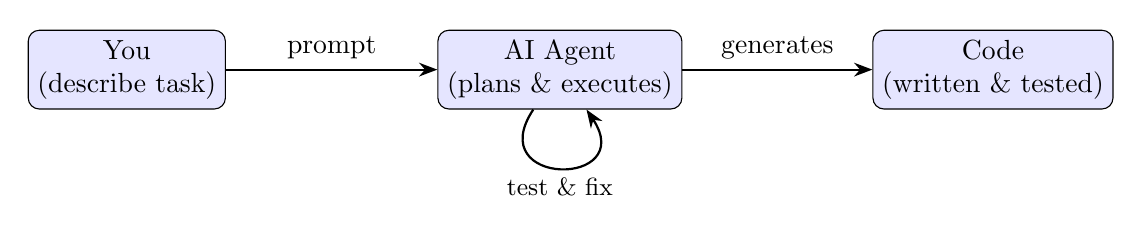
\begin{tikzpicture}[
    box/.style={draw, rounded corners, fill=blue!10, minimum width=2.5cm, minimum height=1cm, align=center},
    arrow/.style={->, thick, >=Stealth}
]
    \node[box] (user) at (0,0) {You\\(describe task)};
    \node[box] (agent) at (5.5,0) {AI Agent\\(plans \& executes)};
    \node[box] (code) at (11,0) {Code\\(written \& tested)};

    \draw[arrow] (user) -- (agent) node[midway, above] {prompt};
    \draw[arrow] (agent) -- (code) node[midway, above] {generates};

    % Self-loop: agent tests, sees errors, fixes, repeats
    \draw[arrow] (agent) .. controls (4.5,-1.5) and (6.5,-1.5) .. node[below,font=\small] {test \& fix} (agent);
\end{tikzpicture}

\vspace{0.5cm}

Unlike simple chatbots, agentic AI can:
\begin{itemize}
    \item Read and navigate your codebase
    \item Write, edit, and delete files
    \item Run commands and tests
    \item Fix errors and iterate until the task is complete
\end{itemize}

\end{frame}

%======================================================================
\section{Setup}
%======================================================================

\begin{frame}{Getting Your API Key}

\textbf{Step 1: Submit HW0 via \href{https://webcourse.cs.technion.ac.il/02360267}{Webcourse}}
\begin{itemize}
    \item Provide your details (name, ID, email)
    \item Provide your partner's details (if working in pairs)
\end{itemize}

\vspace{0.5cm}

\textbf{Step 2: Receive Your API Key}
\begin{itemize}
    \item After HW0 submission, you will receive your personal API key via \href{https://webcourse.cs.technion.ac.il/02360267}{Webcourse}
    \item Key format: \texttt{sk-or-v1-...}
    \item \textbf{Keep this key private!} Do not share it.
\end{itemize}

\vspace{0.5cm}

\textbf{Budget:} \$10 per student --- should suffice for all assignments, but monitor usage!

\end{frame}

%======================================================================
\begin{frame}[fragile]{Configuration: Setting Up Claude Code}

Install Claude Code (macOS/Linux/WSL); 
\begin{minted}[fontsize=\scriptsize,bgcolor=lightgray]{bash}
curl -fsSL https://claude.ai/install.sh | bash
\end{minted}
{\tiny(see \url{https://code.claude.com/docs/en/setup})}
\normalfont
\vspace{0.1cm}

\textbf{Option A:} Shell variables (\texttt{.bashrc}/\texttt{.zshrc}):
\begin{minted}[fontsize=\scriptsize,bgcolor=lightgray]{bash}
export ANTHROPIC_AUTH_TOKEN="sk-or-v1-..."
export ANTHROPIC_API_KEY=""
export ANTHROPIC_BASE_URL="https://openrouter.ai/api"
\end{minted}

\vspace{0.1cm}

\textbf{Option B:} Edit \colorbox{lightgray}{\texttt{\textasciitilde/.claude/settings.json}}:
\begin{minted}[fontsize=\scriptsize,bgcolor=lightgray]{json}
{
  "env": {
    "ANTHROPIC_AUTH_TOKEN": "sk-or-v1-...",
    "ANTHROPIC_API_KEY": "",
    "ANTHROPIC_BASE_URL": "https://openrouter.ai/api",
    "ANTHROPIC_MODEL": "moonshotai/kimi-k2"
  }
}
\end{minted}

\begin{tikzpicture}[remember picture, overlay]
\node[rectangle callout, draw=red, fill=calloutbg, text width=2.8cm, font=\small, align=center,
      callout absolute pointer={([xshift=-1.2cm, yshift=0.8cm]current page.center)}]
      at ([xshift=4cm, yshift=1cm]current page.center) {
    Replace \texttt{...} with your key from \href{https://webcourse.cs.technion.ac.il/02360267}{Webcourse}!
};
\end{tikzpicture}

\end{frame}

%======================================================================
\begin{frame}[fragile]{Checking Your Budget}

To check your remaining budget, run:
\begin{minted}[fontsize=\footnotesize,bgcolor=lightgray]{bash}
curl https://openrouter.ai/api/v1/auth/key \
     -H "Authorization: bearer $ANTHROPIC_AUTH_TOKEN" | jq
\end{minted}

\vspace{0.2cm}

Example output:
\begin{minted}[fontsize=\scriptsize,bgcolor=lightgray]{json}
{
  "data": {
    "label": "sk-or-v1-852...8dd",
    "limit": 10.0,
    "limit_remaining": 9.59,
    "usage": 0.408003788,
    ...
  }
}
\end{minted}

\vspace{0.2cm}

\textbf{Key fields:}
\begin{itemize}
    \item \texttt{usage}: Total amount spent so far (in USD)
    \item \texttt{limit\_remaining}: How much budget you have left
\end{itemize}

\end{frame}

%======================================================================
\begin{frame}[fragile]{IDE Integration}

\textbf{Option 1: Run CLI inside VSCode terminal}
\begin{itemize}
    \item Open new terminal: \colorbox{keybg}{\texttt{Ctrl+Shift+`}}
    \item Run \colorbox{lightgray}{\texttt{claude --model "moonshotai/kimi-k2"}}
    \item Works with either Option A or B configuration
\end{itemize}

\vspace{0.3cm}

\textbf{Option 2: VSCode Extension (recommended)}
\begin{enumerate}
    \item Install ``Claude Code'' from VSCode Marketplace
    \item Configure \colorbox{lightgray}{\texttt{\textasciitilde/.claude/settings.json}} (Option B)
    \item In extension settings: \textbf{Claude Code: Use Terminal} $\rightarrow$ \texttt{integrated}
    \item Click the Claude logo in the sidebar: \raisebox{-0.3em}{\includegraphics[height=1.2em]{figures/claude.png}}
\end{enumerate}

\vspace{0.2cm}

\textbf{Benefits:} Claude sees your open files, workspace context, and you can review changes in VSCode's diff view.

\end{frame}

%======================================================================
\section{Best Practices}
%======================================================================

\begin{frame}{Tips for Effective Prompting}

\textbf{1. Be Specific About Context}
\begin{itemize}
    \item ``Write a Verilog module for a 5-stage pipeline latch''
    \item Not: ``Help me with my assignment''
\end{itemize}

\vspace{0.3cm}

\textbf{2. Break Down Complex Tasks}
\begin{itemize}
    \item Start with the interface/specification
    \item Then implement components incrementally
    \item Test each part before moving on
\end{itemize}

\vspace{0.3cm}

\textbf{3. Provide Examples}
\begin{itemize}
    \item Show input/output examples when possible
    \item Reference existing code patterns in your project
\end{itemize}

\end{frame}

%======================================================================
\begin{frame}{Test-Driven Development with AI}

\textbf{4. Write Tests Early!}
\begin{itemize}
    \item Ask the AI to write tests \textbf{before} or \textbf{alongside} implementation
    \item ``First write a testbench for this module, then implement it''
    \item Verify tests pass at each stage
\end{itemize}

\vspace{0.3cm}

\textbf{5. Run Tests Iteratively}
\begin{itemize}
    \item For complex tasks: run tests after \textbf{every significant change}
    \item Let the AI see test failures and fix them immediately
    \item Don't wait until the end to discover problems!
\end{itemize}

\vspace{0.3cm}

\textbf{6. Use \colorbox{lightgray}{\texttt{CLAUDE.md}} for Project Context}
\begin{itemize}
    \item Create a \colorbox{lightgray}{\texttt{CLAUDE.md}} file in your project root
    \item Document: build commands, test commands, project structure
    \item The AI reads this automatically for context
\end{itemize}

\end{frame}

%======================================================================
\begin{frame}[fragile]{CLAUDE.md: Project Context File}

Create a \colorbox{lightgray}{\texttt{CLAUDE.md}} file in your project root to give Claude persistent context:

\begin{minted}[fontsize=\scriptsize,bgcolor=lightgray]{markdown}
# Build commands
- make: Build the project
- make test: Run all tests
- make debug: Build with debug symbols (-g)
- gdb ./program: Debug with GDB

# Code style
- Use meaningful variable names
- Comment non-obvious bit manipulations

# Project structure
- src/: C source files
- include/: Header files
- tests/: Test cases
\end{minted}

\vspace{0.2cm}

\textbf{Benefits:} Claude reads this automatically $\rightarrow$ better context, fewer mistakes.

\vspace{0.1cm}

{\footnotesize See: \url{https://www.anthropic.com/engineering/claude-code-best-practices}}

\end{frame}

%======================================================================
\begin{frame}{Planning Mode}

For complex tasks, ask the AI to \textbf{plan before implementing}:

\vspace{0.3cm}

\begin{itemize}
    \item Press \colorbox{keybg}{\textbf{Shift+Tab}} to toggle plan mode
    \item Or ask: ``Plan how to implement X before writing code''
    \item The AI will outline its approach for your approval
    \item Review the plan, suggest changes, then let it execute
\end{itemize}

\vspace{0.3cm}

\textbf{Benefits:}
\begin{itemize}
    \item Catch architectural issues early
    \item Ensure the AI understands the requirements
    \item Save tokens/budget by avoiding wrong directions
\end{itemize}

\vspace{0.3cm}

\textbf{Example:} ``Plan how to add branch prediction to the pipeline. Don't write code yet, just explain the approach.''

\end{frame}

%======================================================================
\begin{frame}{Version Control: Rewind and Git}

\textbf{Rewind (CLI only):}
\begin{itemize}
    \item Claude Code CLI has built-in \colorbox{lightgray}{\texttt{/rewind}} to undo changes
    \item Useful if the AI takes a wrong direction
    \item Note: Not available in VSCode extension
\end{itemize}

\vspace{0.3cm}

\textbf{Use Git for Safety:}
\begin{itemize}
    \item \textbf{Commit frequently} before asking AI to make big changes
    \item If something goes wrong: \colorbox{lightgray}{\texttt{git checkout .}} or \colorbox{lightgray}{\texttt{git reset}}
    \item Create branches for experimental features
\end{itemize}

\vspace{0.3cm}

\textbf{Recommended workflow:}
\begin{enumerate}
    \item \colorbox{lightgray}{\texttt{git commit}} your working state
    \item Ask AI to implement feature
    \item If happy: commit the changes
    \item If not: \colorbox{lightgray}{\texttt{git checkout .}} to revert
\end{enumerate}

\end{frame}

%======================================================================
\section{Safety and Permissions}
%======================================================================

\begin{frame}[fragile]{Sandboxing and Permissions}

\textbf{Sandboxing} = OS-level filesystem \& network isolation for safer operation.

\vspace{0.2cm}

\textbf{What it does:}
\begin{itemize}
    \item \textbf{Filesystem:} Write access only to working directory; read access elsewhere
    \item \textbf{Network:} Only approved domains can be accessed
    \item Uses OS primitives (Seatbelt on macOS, bubblewrap on Linux)
\end{itemize}

\vspace{0.2cm}

\textbf{Enable sandboxing:} Type \colorbox{lightgray}{\texttt{/sandbox}} in Claude Code
\begin{itemize}
    \item \textbf{Auto-allow mode:} Commands within sandbox run without prompts
    \item \textbf{Regular mode:} All commands still go through permission flow
\end{itemize}

\vspace{0.2cm}

\textbf{Permissions (separate from sandbox):}
\begin{itemize}
    \item Claude Code asks before running commands
    \item Choose ``Allow once'' or ``Allow always'' when prompted
    \item Pre-approve in \colorbox{lightgray}{\texttt{CLAUDE.md}}: \colorbox{lightgray}{\texttt{- make test}}, \colorbox{lightgray}{\texttt{- gdb ./program}}
\end{itemize}

\end{frame}

%======================================================================
\section{Context Management}
%======================================================================

\begin{frame}{Understanding Context Windows}

\textbf{Context window} = the AI's ``working memory'' for your conversation.

\vspace{0.2cm}

\begin{itemize}
    \item Everything you send (prompts, code, errors) fills the context
    \item The AI also uses context for its ``thinking'' and responses
    \item \textbf{Finite resource:} When full, quality degrades $\rightarrow$ start fresh!
    \item Some models give worse answers as context fills (``context anxiety'')\footnote{See: \url{https://inkeep.com/blog/context-anxiety}}
\end{itemize}

\vspace{0.2cm}

\textbf{Context compaction:} When context fills up, Claude Code automatically summarizes older parts of the conversation to make room. You may see a message like ``Compacting...'' or ``This session is being continued...''
\begin{itemize}
    \item Details from early in the session may become less precise
    \item Important decisions might need to be restated
\end{itemize}

\vspace{0.2cm}

\textbf{Cost implications:} Larger context = more tokens = higher cost.\footnote{Even with KV-cache optimizations, you pay for the full context on each turn.}

\end{frame}

%======================================================================
\begin{frame}{When to Start a Fresh Session}

\textbf{Signs you should start a new session:}
\begin{itemize}
    \item Switching to a completely different task
    \item AI starts making mistakes about earlier code
    \item You've been going for 30+ turns on complex work
    \item Claude Code shows context usage warnings
\end{itemize}

\vspace{0.3cm}

\textbf{How to start fresh:}
\begin{itemize}
    \item \colorbox{lightgray}{\texttt{/clear}} --- clear conversation but stay in same session
    \item \colorbox{lightgray}{\texttt{/new}} --- start a completely new session
    \item Use \colorbox{lightgray}{\texttt{CLAUDE.md}} to preserve project knowledge across sessions
    \item Commit your work before starting new sessions
\end{itemize}

\vspace{0.3cm}

\textcolor{codegreen}{\textbf{Tip:}} Don't try to do everything in one session --- shorter, focused sessions work better.

\end{frame}

%======================================================================
\begin{frame}{Advanced: Skills and Subagents}

Claude Code has features that help manage context more efficiently:

\vspace{0.3cm}

\textbf{Subagents:}
\begin{itemize}
    \item Separate AI instances with their own context windows
    \item Main agent delegates tasks, gets summarized results back
    \item Reduces context bloat in your main conversation
\end{itemize}

\vspace{0.3cm}

\textbf{Skills:}
\begin{itemize}
    \item Reusable prompt templates for common tasks
    \item Encapsulate complex workflows into simple commands
    \item Keep your main context clean
\end{itemize}

\vspace{0.3cm}

{\footnotesize
Learn more:\\
\url{https://code.claude.com/docs/en/sub-agents}\\
\url{https://code.claude.com/docs/en/skills}
}

\end{frame}

%======================================================================
\section{Workflow Examples}
%======================================================================

\begin{frame}[fragile]{Example Workflow}

\textbf{Task:} Implement a bypass unit for the pipeline

\vspace{0.3cm}

\begin{minted}[fontsize=\scriptsize,bgcolor=lightgray]{text}
You: "First, write a testbench for a bypass/forwarding unit that
     detects RAW hazards. Then implement the unit to pass the tests."

Claude: [writes testbench first, then implements bypass_unit.v,
         runs tests, sees failures, fixes logic, re-runs tests...]

You: "The forwarding from MEM stage isn't working for load
     instructions. Here's the error: ..."

Claude: [debugs, identifies the issue, fixes the logic, runs tests
         again until they pass...]
\end{minted}

\vspace{0.3cm}

The AI handles the implementation details while you focus on understanding the architecture.

\end{frame}

%======================================================================
\begin{frame}{Common Pitfalls to Avoid}

\begin{itemize}
    \item[\textcolor{red}{\textbf{X}}] \textbf{Blind trust:} Always verify the AI's output
    \item[\textcolor{red}{\textbf{X}}] \textbf{Vague prompts:} ``Make it work'' $\rightarrow$ be specific
    \item[\textcolor{red}{\textbf{X}}] \textbf{Ignoring errors:} Feed error messages back to the AI
    \item[\textcolor{red}{\textbf{X}}] \textbf{One giant prompt:} Break tasks into smaller steps
    \item[\textcolor{red}{\textbf{X}}] \textbf{Testing at the end:} Write and run tests early!
\end{itemize}

\vspace{0.5cm}

\begin{itemize}
    \item[\textcolor{codegreen}{\textbf{\checkmark}}] \textbf{Understand everything:} Ask for explanations
    \item[\textcolor{codegreen}{\textbf{\checkmark}}] \textbf{Iterative refinement:} Build up complexity gradually
    \item[\textcolor{codegreen}{\textbf{\checkmark}}] \textbf{Commit often:} Use git as your safety net
    \item[\textcolor{codegreen}{\textbf{\checkmark}}] \textbf{Plan first:} For complex tasks, review the plan
\end{itemize}

\end{frame}

%======================================================================
\begin{frame}[fragile]{Troubleshooting}

\textbf{``It's not working!''} --- Check these first:

\vspace{0.3cm}

\begin{enumerate}
    \item \textbf{Wrong model?} Check the status bar --- should say \texttt{kimi-k2}
    \begin{itemize}
        \item If \texttt{claude-sonnet} $\rightarrow$ check config (or you have your own Anthropic account)
    \end{itemize}

    \item \textbf{API key not set?} Run: \colorbox{lightgray}{\texttt{echo \$ANTHROPIC\_AUTH\_TOKEN}}
    \begin{itemize}
        \item Should print your \texttt{sk-or-v1-...} key
        \item Empty? $\rightarrow$ Re-check your shell config or \colorbox{lightgray}{\texttt{settings.json}}
    \end{itemize}

    \item \textbf{Out of budget?} Check with the curl command from earlier slides

    \item \textbf{VSCode extension not connecting?}
    \begin{itemize}
        \item Restart VSCode after editing \colorbox{lightgray}{\texttt{\textasciitilde/.claude/settings.json}}
        \item Make sure ``Use Terminal'' is set to \texttt{integrated}
    \end{itemize}

    \item \textbf{Feature not working?} Some Claude Code features (context indicators, etc.) may not work with non-Claude models --- this is expected.
\end{enumerate}

\end{frame}

%======================================================================
\section{Policies}
%======================================================================

\begin{frame}{Academic Integrity}

\textbf{Using LLMs is allowed and encouraged for this pilot.}

\vspace{0.4cm}

However:
\begin{itemize}
    \item You must \textbf{understand} all code you submit
    \item You may be asked to \textbf{explain} your implementation
    \item \textbf{Do not share} your API key with others
    \item \textbf{Do not share} solutions with other groups
\end{itemize}

\vspace{0.4cm}

\textbf{Important:} The \textbf{exam will likely include questions} about the subjects covered in the programming assignments. Make sure you understand the code you write, not just how to use the AI tools!

\vspace{0.4cm}

The goal is to learn \textbf{computer architecture concepts} --- the AI is a tool to help you get there.

\end{frame}

%======================================================================
\begin{frame}{Summary}

\textbf{Setup:} Submit HW0 $\rightarrow$ get API key $\rightarrow$ configure Claude Code

\vspace{0.3cm}

\textbf{Workflow:}
\begin{itemize}
    \item Write tests early, run iteratively
    \item Plan first, then implement
    \item Commit before big changes
    \item Start fresh sessions for new tasks
\end{itemize}

\vspace{0.3cm}

\textbf{Remember:} Understand everything you submit!

\vspace{0.4cm}

\textbf{Questions?} \hfill {\footnotesize Docs: \url{https://code.claude.com/docs/en/setup}}

\end{frame}

\end{document}
